\documentclass{standalone}
\begin{document}
	\subsection{Pipeline Structure}
	
	In the end the pipeline structure is divided in three main blocks as displaied in \figurename\,\ref{fig:Pipeline} : 
	\begin{itemize}
		\item Pre-Processing and lung extraction 
		\item Training 
		\item Labeling
	\end{itemize}
	
		
	\begin{figure}\label{fig:Pipeline}
		\centering 
		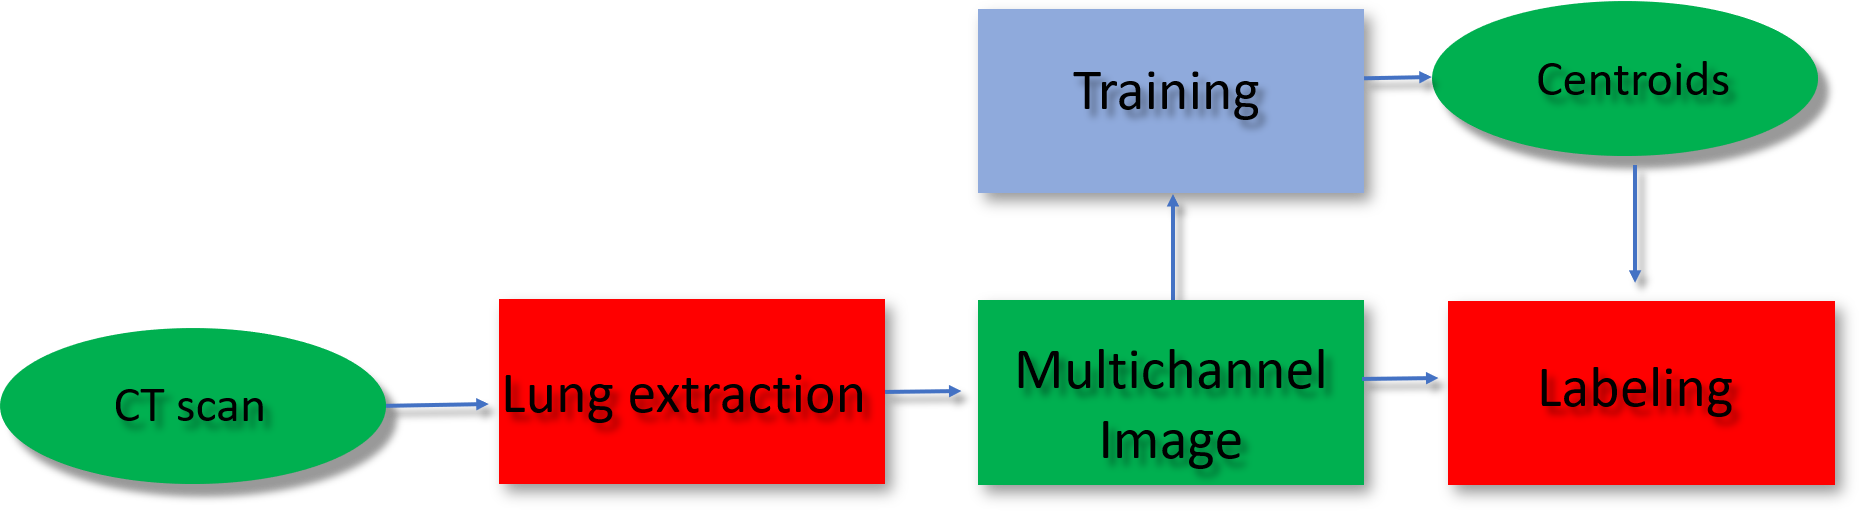
\includegraphics[width=.3\textwidth]{Pipeline.png}
		\caption{Flow chart of the main structure of the developed pipeline. The training process, which allows the estimation of the centroids, is perfromed only one time.}
	\end{figure} 

	\subsubsection*{Pre Processing and Lung Extraction}
	
	Before starting with the actual segmentation, some pre-processing steps are required. First of all we have to mange the input HU to remove all the unwanted regions and manage some artifacts like metallic one. 
	Once we have pre-processed the input volume, we can isolate the lung regions, by removing all the body regions and the extra lung organs, like heart and intestine, which are included into the CT scan. 
	In this way it is possible to focus the segmentation only on the region of interest, avoiding the creation of false positives.   
	
	\subsubsection*{Training}
	
	This step is the most time consuming and computational expansive of the whole pipeline, but it will be run only one time. This step involves the estimation of the centroids for each of the lung structures. It will be run on a lot of different patients in order to obtain a statistical rapresentation, but some results have shown that we can obtain similar results by performing the training only on one image in which each structure is rapresented by a suitable amount of pixels. 
	Once we have estimated the centroids matrix, this process will not be performed again, so doesn't appears on the pipeline of the actual segmentation and doesn't affect the segmentation time. 
	
	\subsection*{Labeling}
	
	This step involves the actual segmentation. The script which perform it requires as inputs the image after the lung extraction, and the previously estimated centroids. This block of the pipeline simply assign each voxel to the cluster corresponding to the nearest centroids. and the end of the procedure only the cluster corresponding to the GGO are provided. In this way we are performing a pixel classification thechniques by assign regions to a particular labels according only to intensities information, without exploiting spatial information: this allow us to group on the same cluster objects that are spatially disconnected as often happen in medical imaging field
	
	So in the end, once we have estimated the centroids, the segmentation pipeline will results of only two steps, as shown in \figurename\,\ref{fig:FinalPipeline} , in which we can observe the flowchart of each step with an image that shown the partial results.
	
	
	\begin{figure}\label{fig:FinalPipeline}
		\centering
			
\includegraphics[width=.3\textwidth]{PlaceHolder.png}
			\caption{PlaceHolder}
	\end{figure}
	
	
	
\end{document}